\documentclass[aspectratio=169]{beamer}
\usetheme{Madrid}
\usecolortheme{seahorse}
\usepackage{tikz}
\usetikzlibrary{shapes,arrows,positioning,trees,shadows,calc}
\usepackage{amsmath}
\usepackage{amssymb}

\setbeamertemplate{navigation symbols}{}
\setbeamercolor{frametitle}{fg=white,bg=blue!70!black}
\setbeamercolor{block title}{bg=blue!60,fg=white}

\title{Decision Trees with Dirichlet Distribution}
\author{}
\date{}

\begin{document}

% Slide 1: Decision Tree with Dirichlet Distribution
\begin{frame}{Decision Tree Prediction with Dirichlet Distribution}
\begin{columns}[T]
\begin{column}{0.48\textwidth}
\centering
\vspace{-0.5cm}
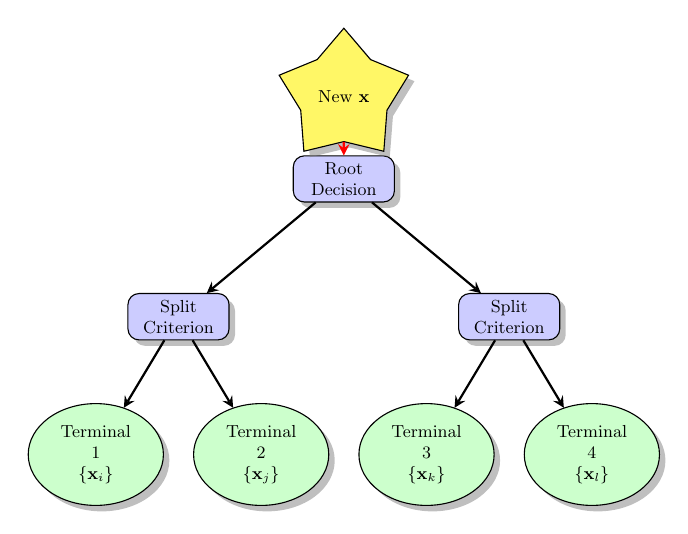
\begin{tikzpicture}[
    scale=0.7,
    every node/.style={transform shape},
    decision/.style={rectangle, draw, fill=blue!20, text width=1.6cm, align=center, rounded corners, drop shadow, font=\small},
    terminal/.style={ellipse, draw, fill=green!20, text width=1.5cm, align=center, drop shadow, font=\small},
    arrow/.style={->, >=stealth, thick}
]

% Root node
\node[decision] (root) at (0,0) {Root\\Decision};

% Level 1
\node[decision] (left1) at (-3,-2.5) {Split\\Criterion};
\node[decision] (right1) at (3,-2.5) {Split\\Criterion};

% Terminal nodes
\node[terminal] (term1) at (-4.5,-5) {Terminal 1\\$\{\mathbf{x}_i\}$};
\node[terminal] (term2) at (-1.5,-5) {Terminal 2\\$\{\mathbf{x}_j\}$};
\node[terminal] (term3) at (1.5,-5) {Terminal 3\\$\{\mathbf{x}_k\}$};
\node[terminal] (term4) at (4.5,-5) {Terminal 4\\$\{\mathbf{x}_l\}$};

% Arrows
\draw[arrow] (root) -- (left1);
\draw[arrow] (root) -- (right1);
\draw[arrow] (left1) -- (term1);
\draw[arrow] (left1) -- (term2);
\draw[arrow] (right1) -- (term3);
\draw[arrow] (right1) -- (term4);

% New observation
\node[draw, star, star points=5, fill=yellow!60, drop shadow, font=\small] (new) at (0,1.5) {New $\mathbf{x}$};
\draw[->, >=stealth, thick, red, dashed] (new) -- (root);

\end{tikzpicture}
\end{column}

\begin{column}{0.52\textwidth}
\vspace{-0.3cm}
\begin{block}{Prediction Process}
{\small
\begin{enumerate}
    \item \textbf{Traverse} tree with new $\mathbf{x}$
    \item \textbf{Locate} terminal node
    \item \textbf{Predict} using:
\end{enumerate}
}
\end{block}

\vspace{0.2cm}

\begin{alertblock}{Two Prediction Options}
{\small
\textbf{Option 1:} Mean
$\hat{y} = \frac{1}{n}\sum_{i=1}^{n} y_i$

\textbf{Option 2:} Dirichlet params
$\hat{y} = f(\boldsymbol{\alpha})$
}
{\footnotesize where $\boldsymbol{\alpha}$ are estimated parameters}
\end{alertblock}
\end{column}
\end{columns}
\end{frame}

% Slide 2: Random Forest
\begin{frame}{Random Forest: Ensemble of Decision Trees}
\begin{columns}[T]
\begin{column}{0.48\textwidth}
\centering
\vspace{-0.3cm}
\begin{tikzpicture}[scale=0.55, every node/.style={transform shape}]

% Three small trees
\foreach \x/\col in {0/blue, 3.5/green, 7/orange} {
    % Tree \x
    \node[rectangle, draw, fill=\col!20, rounded corners, font=\tiny] (r\x) at (\x,3) {Tree};
    \node[circle, draw, fill=\col!15, inner sep=1pt] (l\x) at (\x-0.6,2.2) {};
    \node[circle, draw, fill=\col!15, inner sep=1pt] (rr\x) at (\x+0.6,2.2) {};
    \node[circle, draw, fill=\col!30, inner sep=1pt] (ll\x) at (\x-0.9,1.4) {};
    \node[circle, draw, fill=\col!30, inner sep=1pt] (lr\x) at (\x-0.3,1.4) {};
    \node[circle, draw, fill=\col!30, inner sep=1pt] (rl\x) at (\x+0.3,1.4) {};
    \node[circle, draw, fill=\col!30, inner sep=1pt] (rrr\x) at (\x+0.9,1.4) {};
    
    \draw (r\x) -- (l\x);
    \draw (r\x) -- (rr\x);
    \draw (l\x) -- (ll\x);
    \draw (l\x) -- (lr\x);
    \draw (rr\x) -- (rl\x);
    \draw (rr\x) -- (rrr\x);
    
    % Predictions
    \node[below=0.05cm of ll\x, font=\tiny] {$\hat{y}_t$};
}

% New observation at top
\node[draw, star, star points=5, fill=yellow!60, drop shadow, font=\tiny] (new) at (3.5,4.2) {New $\mathbf{x}$};

% Arrows from new to trees
\draw[->, >=stealth, thick, dashed, red] (new) -- (r0);
\draw[->, >=stealth, thick, dashed, red] (new) -- (r3.5);
\draw[->, >=stealth, thick, dashed, red] (new) -- (r7);

% Dots indicating more trees
\node at (8.5,2.5) {$\cdots$};
\node at (8.5,1.8) {\tiny $T$ trees};

% Aggregation
\node[rectangle, draw, fill=purple!20, rounded corners, drop shadow, text width=2.5cm, align=center, font=\small] (agg) at (3.5,0.2) {\textbf{Average}\\{\footnotesize $\hat{y} = \frac{1}{T}\sum_{t=1}^{T}\hat{y}_t$}};

% Arrow to aggregation
\draw[->, >=stealth, ultra thick, purple] (3.5,1) -- (agg);

\end{tikzpicture}
\end{column}

\begin{column}{0.52\textwidth}
\vspace{-0.3cm}
\begin{block}{Random Forest Algorithm}
{\small
\textbf{For each tree} $t = 1, \ldots, T$:
\begin{enumerate}
    \item Build tree on bootstrap sample
    \item Use Dirichlet distribution
    \item Predict: $\hat{y}_t$
\end{enumerate}
}
\end{block}

\vspace{0.2cm}

\begin{exampleblock}{Final Prediction}
{\small
Aggregate from all trees:
$\boxed{\hat{y}_{\text{forest}} = \frac{1}{T}\sum_{t=1}^{T} \hat{y}_t}$
}
\vspace{0.1cm}
{\small
\textbf{Benefits:}
\begin{itemize}
    \item Reduced variance
    \item Improved generalization
    \item Robust predictions
\end{itemize}
}
\end{exampleblock}
\end{column}
\end{columns}
\end{frame}

\end{document}